\documentclass[11pt,a4paper]{article}

% ---------------------------------------------------------
% Packages
% ---------------------------------------------------------
\usepackage[margin=1.5cm]{geometry}
\usepackage{tikz}
\usetikzlibrary{calendar}
\usepackage{xcolor}
\usepackage{csvsimple}
\usepackage{ifthen}
\usepackage{etoolbox}
\usepackage{array}
\usepackage{longtable}

% ---------------------------------------------------------
% Colors
% ---------------------------------------------------------
\definecolor{calendarblue}{RGB}{40,100,180}
\definecolor{calendarlight}{RGB}{235,242,250}
\definecolor{weekend}{RGB}{245,245,245}
\definecolor{activitycolor}{RGB}{220,235,250}

% ---------------------------------------------------------
% Read activities from CSV
% ---------------------------------------------------------
% Store activities for each date in commands such as:
% \activities@2026-09-07

\makeatletter

\newcommand{\addactivity}[4]{%
    \expandafter\gdef\csname activities@#1\endcsname{%
        \textbf{#2} -- \textbf{#3}\\
        #4\par\vspace{2pt}%
    }%
}

% Default value for dates with no activities
\newcommand{\getactivities}[1]{%
    \ifcsname activities@#1\endcsname
        \csname activities@#1\endcsname
    \else
        \textcolor{gray}{No activities}
    \fi
}

% Read CSV and create commands
\csvreader[
    head to column names,
    late after line=%
]{activities.csv}{}{%
    \addactivity{\date}{\time}{\activity}{\description}%
}

\makeatother

% ---------------------------------------------------------
% Calendar styling
% ---------------------------------------------------------
\tikzset{
    calendarbox/.style={
        draw=gray!60,
        rectangle,
        minimum width=3.0cm,
        minimum height=3.0cm,
        anchor=north west,
        inner sep=5pt,
        align=left
    },
    daynumber/.style={
        font=\bfseries\large,
        text=calendarblue
    }
}

% ---------------------------------------------------------
% Calendar parameters
% ---------------------------------------------------------
\newcommand{\CalendarYear}{2026}
\newcommand{\CalendarMonth}{9}

% ---------------------------------------------------------
% Create calendar
% ---------------------------------------------------------
\begin{document}

\begin{center}
    {\Huge\bfseries September 2026}\\[5pt]
    {\large Activity Calendar}
\end{center}

\vspace{0.5cm}

\begin{center}

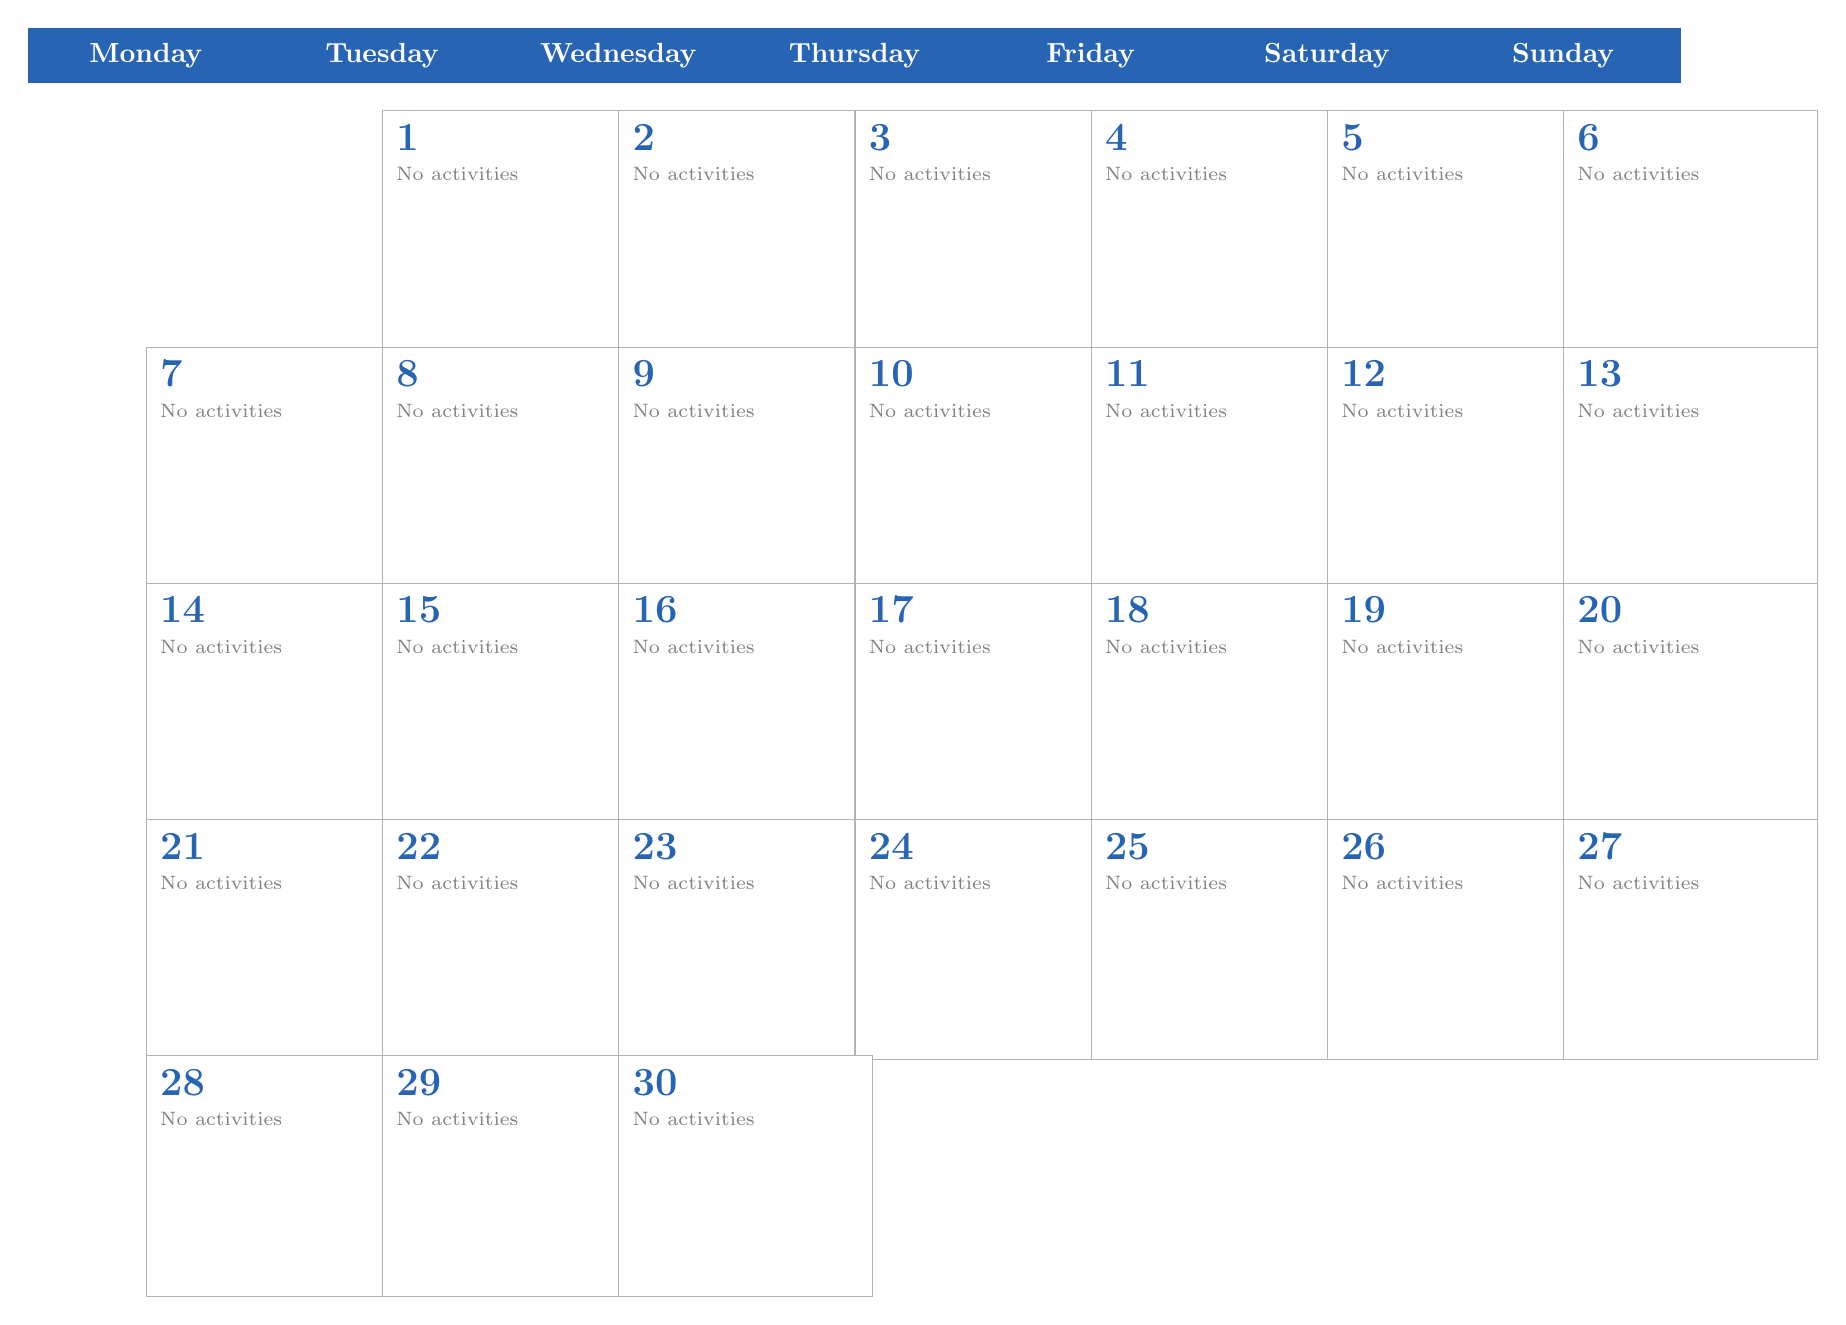
\begin{tikzpicture}

% ---------------------------------------------------------
% Day names
% ---------------------------------------------------------
\foreach \day [count=\i from 0] in
    {Monday,Tuesday,Wednesday,Thursday,Friday,Saturday,Sunday}
{
    \node[
        minimum width=3.0cm,
        minimum height=0.7cm,
        fill=calendarblue,
        text=white,
        font=\bfseries
    ]
    at (\i*3.0cm,0)
    {\day};
}

% ---------------------------------------------------------
% Calendar days
% ---------------------------------------------------------

% September 2026 starts on Tuesday.
% Therefore Monday is column 0 and Tuesday is column 1.

\foreach \d/\col/\row in {
    1/1/0,
    2/2/0,
    3/3/0,
    4/4/0,
    5/5/0,
    6/6/0,
    7/0/1,
    8/1/1,
    9/2/1,
    10/3/1,
    11/4/1,
    12/5/1,
    13/6/1,
    14/0/2,
    15/1/2,
    16/2/2,
    17/3/2,
    18/4/2,
    19/5/2,
    20/6/2,
    21/0/3,
    22/1/3,
    23/2/3,
    24/3/3,
    25/4/3,
    26/5/3,
    27/6/3,
    28/0/4,
    29/1/4,
    30/2/4
}
{
    % Calculate coordinates
    \pgfmathsetmacro{\x}{\col*3.0}
    \pgfmathsetmacro{\y}{-0.7-\row*3.0}

    % Date string
    \edef\datestring{\CalendarYear-\CalendarMonth-\d}

    % Day box
    \node[
        calendarbox,
        fill=white
    ]
    at (\x cm,\y cm)
    {%
        \begin{minipage}[t][2.7cm][t]{2.75cm}
            \raggedright

            % Day number
            \textcolor{calendarblue}{\Large\bfseries \d}

            \vspace{3pt}

            % Activities
            \scriptsize
            \getactivities{\datestring}

        \end{minipage}
    };
}

\end{tikzpicture}

\end{center}

\end{document}